\documentclass[12pt]{amsart}
\usepackage{geometry} % see geometry.pdf on how to lay out the page. There's lots.
\usepackage{graphicx}	% Including figure files
\usepackage{amsmath}	% Advanced maths commands
\usepackage{amssymb}	% Extra maths symbols
\usepackage{hyperref}
\usepackage{float}
\floatplacement{figure}{H}
\floatplacement{table}{H} 
\geometry{a4paper} % or letter or a5paper or ... etc

\title{CSE 546: Machine Learning Homework 3}
\author{David P. Fleming}
\date{November xxx$^{th}$, 2016}

%%% BEGIN DOCUMENT
\begin{document}

\maketitle
\tableofcontents

\section*{Introduction}

Please note that a copy of all the code I wrote to answer the questions in this assignment are included in my submission but also located online at \url{https://github.com/dflemin3/CSE_546/tree/master/HW3}.  Some scripts require data, such as MNIST data, to run to completion and were not included on my github due to file size constraints.  The MNIST data is included in the {\tt Data} directory as python {\tt .pkl} files as this compressed format gave me quicker load times for my scripts.

Overall, my code is structured as follows:  There are three main directories included in my submission: {\tt DML}, {\tt Data} and {\tt HW3}. {\tt HW3} contains all the scripts used to run my analysis.  For example to reproduce the answer for Question 1.2, one would run {\tt python hw3$\_1.2.py$}.  All scripts have relative file paths so the code should run and have detailed comments to describe functionality.  In addition, the scripts have flags near the top to control functionality.  By default, I set all flags to true so the script performs the entire analysis and plotting.  The {\tt Data} directory contains both the MNIST dataset. The grader should be able to run my homework scripts without altering this directory.  

The {\tt DML} directory contains all the auxiliary files used to do the computations in the homework scripts and has a logical hierarchy.  For example, the directory {\tt optimization} contains the file {\tt gradient$\_$descent.py} while contains both my batch gradient descent and stochastic gradient descent implementations.  The directory {\tt data$\_$processing} contains the script {\tt mnist$\_$utils.py} which contains my functions used to load and work with the MNIST data.  The directory {\tt classification} contains the file {\tt classifier$\_$utils.py} which contains all things related to binary and softmax classification including the gradients for each respective method for use with a gradient descent algorithm.  The {\tt validation} subdirectory contains {\tt validation.py}.  This file contains all my loss functions such as 0/1 loss and also my implementations for regularization paths for both linear regression and logistic and softmax classification using gradient descent.  Finally, the {\tt regression} directory contains all utilities for a normal or multi-class regression.  In particular, this directory contains the file where my ridge regression implementation lives, {\tt ridge$\_$utils.py}. 

In each section, I try to be explicit with what files I used to perform the computation including the path from the {\tt DML} directory for ease of grading.

%%% QUESTION 0  %%%
\section*{Question 0: Collaborators}
I collaborated with Matt Wilde, Serena Liu, and Janet Matsen for various questions on this assignment.

%%% QUESTION 1 %%%

\section*{Question 1: PCA and reconstruction}

In this question, I derive matrix algebra relations and I use my PCA implementation to reduce the dimensionality of the MNIST dataset and visualize the results.  The code used to solve this question is in the following attached files: {\tt hw3$\_$1.2.py, hw3$\_$1.3.py, hw3$\_$1.4.py} in the {\tt HW3} directory and {\tt classification/classifier$\_$utils.py, regression/regression$\_$utils.py, validation/validation.py, data$\_$processing/mnist$\_$utils.py} in the {\tt DML} directory.

\subsection*{1.0: Details of my PCA implementation}

My PCA implementation performs a SVD on the MNIST training datat $X$ to derive the principal components and the eigenvectors of the empirical covariance matrix, Eqn.~\ref{eqn:sigma}.   Performing PCA using a SVD gives me the following matrices: $u$, $s$, and $v$ where the columns of $v$ are the eigenvectors of Eqn.~\ref{eqn:sigma}.  The eigenvalues of Eqn.~\ref{eqn:sigma} are given by the square of the singular values divided by the length of the dataset, $\lambda = s^2/N$.

To transform the dataset to a lower dimensional space using the first $l$ principal components, the first $l$ columns of $v$, I evaluate
\begin{equation} \label{eqn:pca_transform}
X_{trans} = Xv
\end{equation}
since $X$ is $N \times d$ and the truncated $v$ is $d \times l$ resulting in a lower-dimensional $N \times l$ $X_{trans}$.  I reproject my lower-dimensional transformed data back into``physical'' space via
\begin{equation} \label{eqn:pca_inverse_transform}
X_{approx} = X_{trans}v^T
\end{equation} 
since $X_{trans}$ is $N \times l$ and $v^T$ is $l \times d$ resulting in a $N \times d$ matrix.  Note that $X_{approx} \neq X$ for $l < d$ principal components since using less than the total feature number of principal components instead yields an approximation of the original data when projected back into the original space.

Note that for all questions, I first centered the training data before running PCA.  Specifically, for each feature (column) of $X$, I subtracted off its mean.  In addition to the textbook suggesting this as a good practice, I found that it yielded better performance and hence do so for all PCA questions in this homework set in less explicitly stated otherwise.

\subsection*{1.1: Matrix Algebra Review}

\begin{equation} \label{eqn:sigma}
\Sigma = \frac{1}{N}\sum_i x_i x_i^T
\end{equation}

TODO

\subsection*{1.2: PCA}

Here I performed PCA on the MNIST training data and retained the first 50 principal components and singular values.  The code used to answer this question is located in files: {\tt hw3$\_$1.2.py} in the {\tt HW3} directory and {\tt pca/pca.py} in the {\tt DML} directory.

\subsubsection*{1.2.1}

The eigenvalues $\lambda_1, \lambda_2, \lambda_{10}, \lambda_{30}, \lambda_{50}$ are 332719.1, 243279.9, 80808.5, 23685.7, and 11035.3, respectively. The sum of all eigenvalues is 3428445.4.  Again, I calculate $\lambda = s^2/N$ for singular value $s$ and dataset size $N$.

\subsubsection*{1.2.2}

I plot the fractional reconstruction error for $k \in [1,50]$ for the $k$ principal components in Fig.~\ref{fig:frac_rec_error}.  The fractional reconstruction error is defined as
\begin{equation} \label{eqn:frac_rec_error}
F = 1 - \frac{\sum_{i=1}^k \lambda_i}{\sum_{i=1}^d \lambda_i}
\end{equation}
for $d$ total features and $k$ principal components.  Note how the first principal component is the largest eigenvalue as shown above.
 
\begin{figure}[H]
	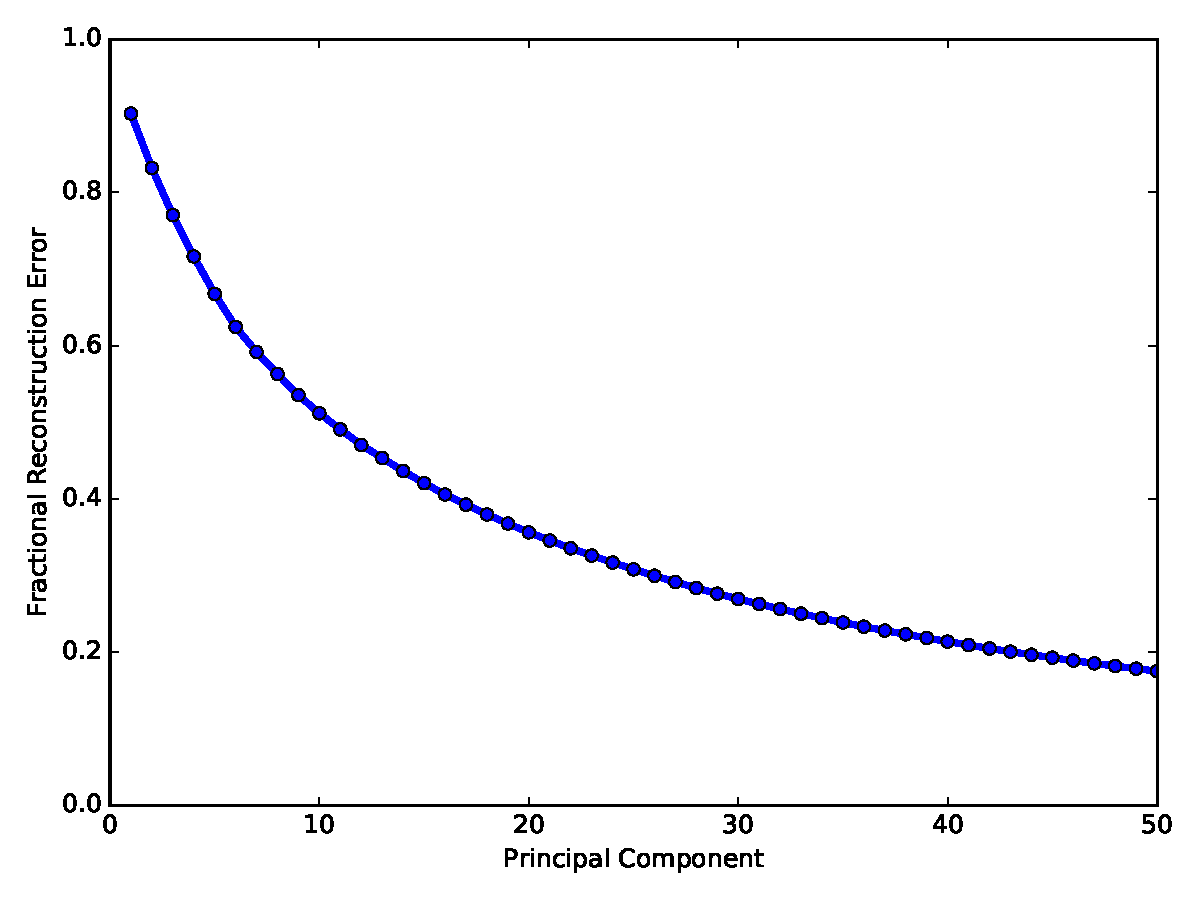
\includegraphics[width=\columnwidth]{fractional_rec_error.pdf}
    \caption{Fractional reconstruction error as a function of $k$ principal components out of $d$ total dimensions for $k \in [1,50]$.}
    \label{fig:frac_rec_error}
\end{figure}


\subsubsection*{1.2.3}

The first eigenvalue, and its corresponding principal component, represent the component of the data that captures the most variance.  That is, the first eigenvalue represents the mean covariance of the data.

\subsubsection*{1.2.4}

I plot the fractional reconstruction error for $k \in [2,50]$ for the $k$ principal components in Fig.~\ref{fig:frac_rec_error_sans_mean}.  As expected, we see that the absence of the first eigenvalue demonstrates its importance.

\begin{figure}[H]
	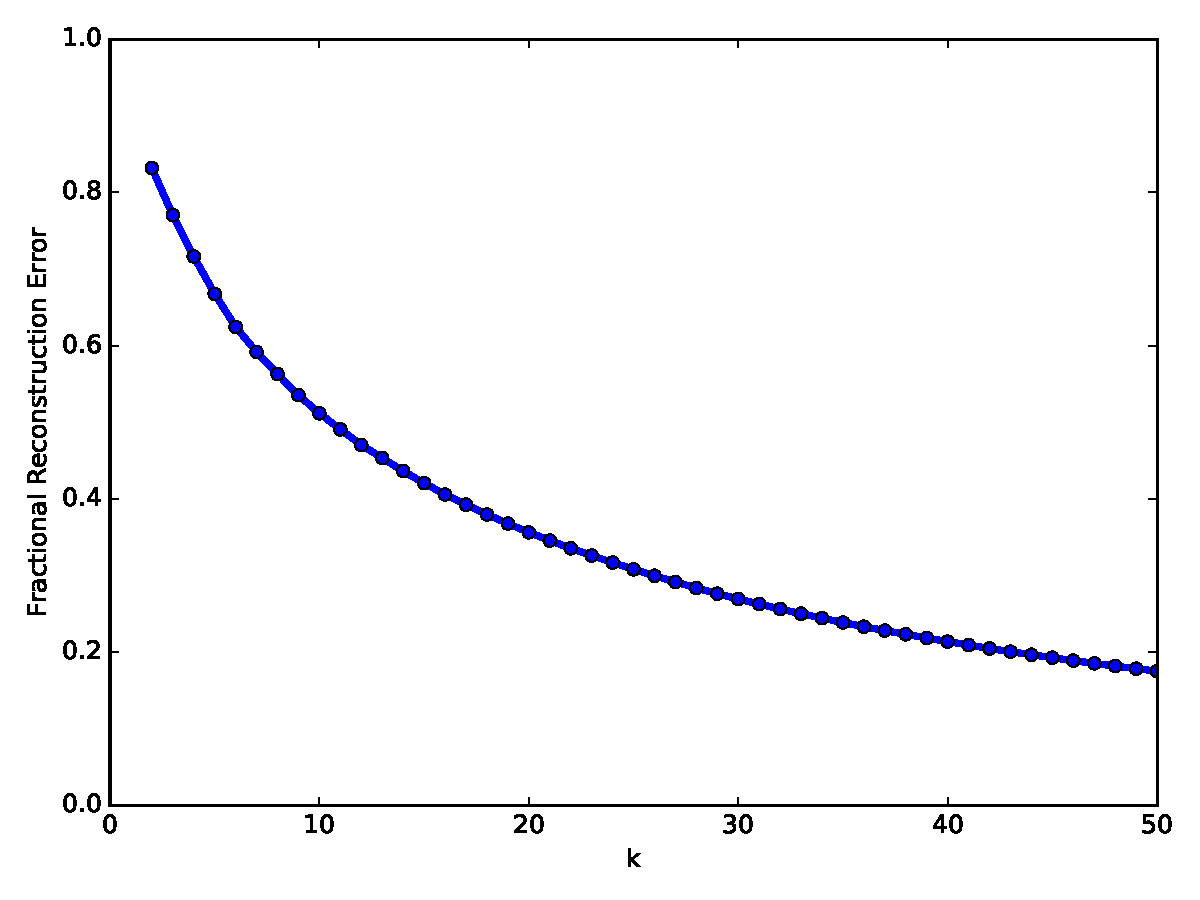
\includegraphics[width=\columnwidth]{fractional_rec_error_sans_mean.pdf}
    \caption{Fractional reconstruction error as a function of $k$ principal components out of $d$ total dimensions for $k \in [2,50]$.}
    \label{fig:frac_rec_error_sans_mean}
\end{figure}

\subsection*{1.3: Visualization of the Eigen-Directions}

\subsubsection*{1.3.1}

I plot the first 16 eigenvectors in Fig.~\ref{fig:eigendirections} as images.  To do so, I reshaped each vector into a $28 \times 28$ pixel image.  For each image, I also annotate it with its number such that the second eigendirection would have a ``2'' in its image.  I plotted 16 instead of 10 since 16 gives a nice symmetric collection of subplots.

\begin{figure}[H]
	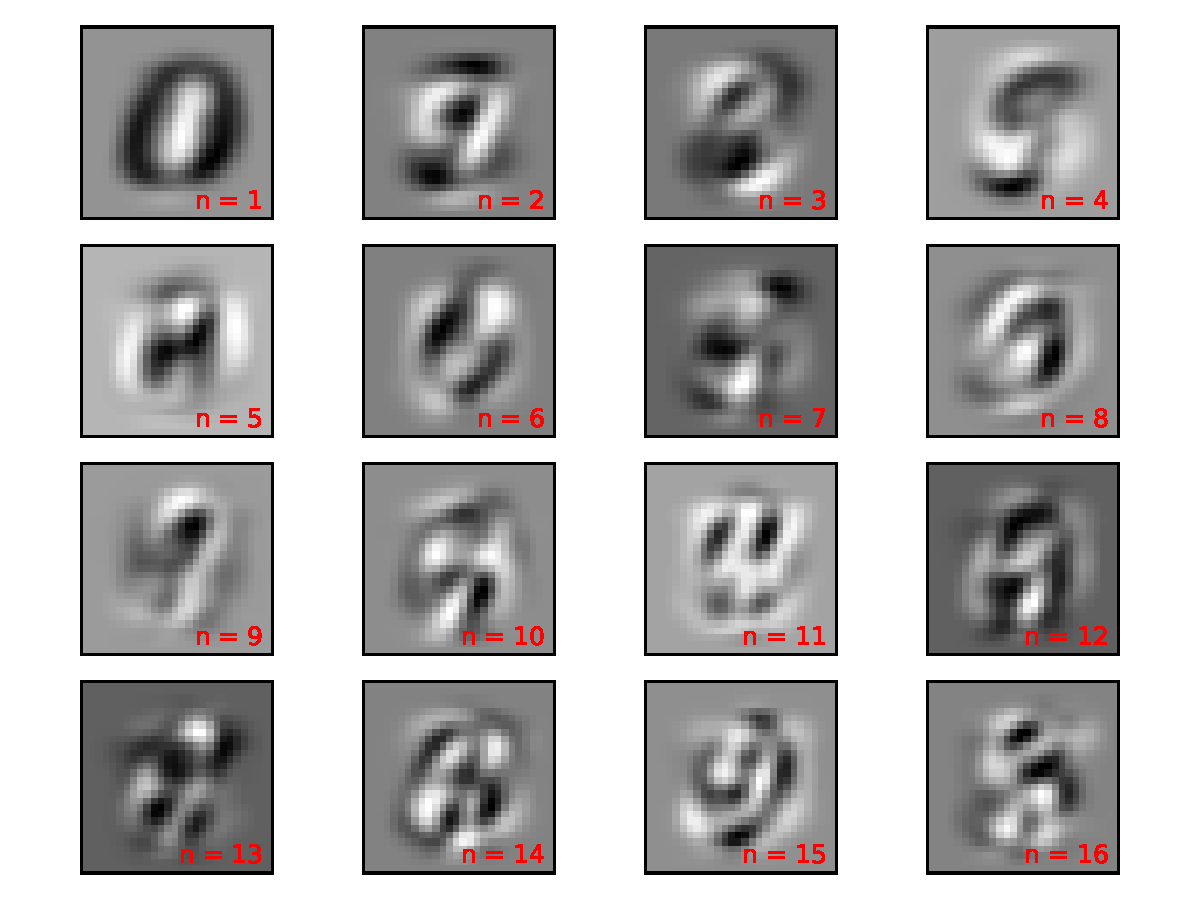
\includegraphics[width=\columnwidth]{eigendirections.pdf}
    \caption{Visualization of the first 16 eigendirections as $28 \times 28$ pixel images.  The respective eigendirection number is given in red in a subplot's lower righthand corner.}
    \label{fig:eigendirections}
\end{figure}

\subsubsection*{1.3.2}

Each individual eigendirection, or principal component, captures a fundamental basis vector in an orthogonal set which each explain a decreasing variation in the data with increasing principal component number.  That is, the first principal component accounts for the most variability in the data while subsequent components account for less and less variability.  This intuitive picture makes sense upon examining Fig.~\ref{fig:eigendirections}.  The first four components themselves appear to represent the numbers 0, 9, 3, and 5, respectively.  Although the components do not explicitly represent those numbers, instead the represent characteristics of numbers in the dataset that are commonly shared.  Many of the digits share features with 9, 3, and 5, for example, like their openings on the lefthand side of the digit and the solid vertical line on the righthand side of the digit.

\subsection*{1.4: Visualization and Reconstruction}

\subsubsection*{1.4.1}
Here, I choose 6 unique digits from the MNIST training set and plot them in Fig.~\ref{fig:mnist_digits}.  I annotate each digit's image with its label in the lower-righthand corner.  I chose 6 digits instead of 5 for symmetry's sake.
\begin{figure}[H]
	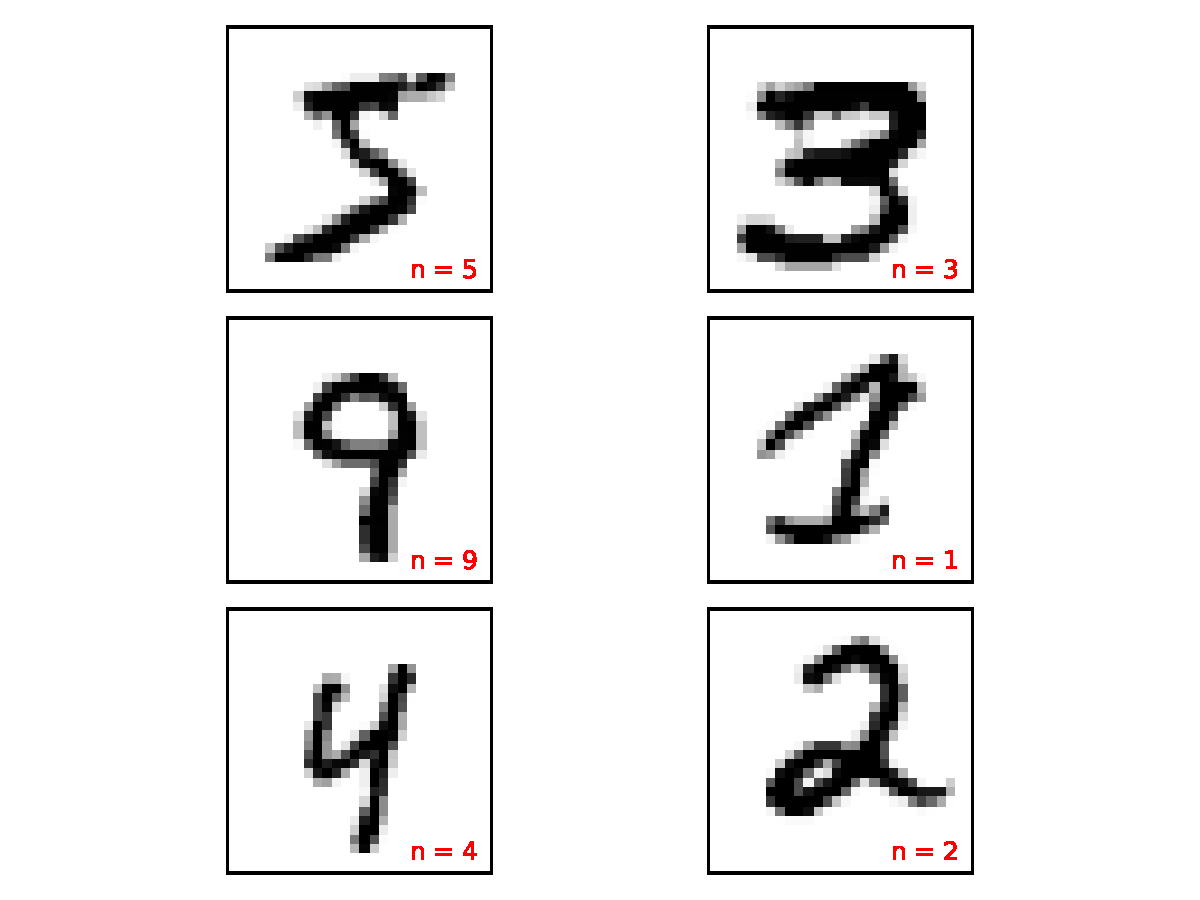
\includegraphics[width=\columnwidth]{mnist_digits.pdf}
    \caption{Visualization of 6 random, unique digits from the MNIST training set.  The image label is displayed in red in the lower-righthand corner of each image.}
    \label{fig:mnist_digits}
\end{figure}

\subsubsection*{1.4.2}

Now I perform PCA on the MNIST training set keeping the first 100 principal components.  Using this fit and the same digits displayed in Fig.~\ref{fig:mnist_digits}, I reconstruct the digits using 2, 5, 10, 20, 50, and 100 principal components using the reconstruction $X_{recon} = Xvv^T$.  The reconstructions are displayed in Fig.~\ref{fig:recon_5}, Fig.~\ref{fig:recon_3}, Fig.~\ref{fig:recon_9}, Fig.~\ref{fig:recon_1}, Fig.~\ref{fig:recon_2}, and Fig.~\ref{fig:recon_4}.  For each reconstructed image using $k$ principal components, $k$ is shown in red in the lower-righthand corner.

\begin{figure}[H]
	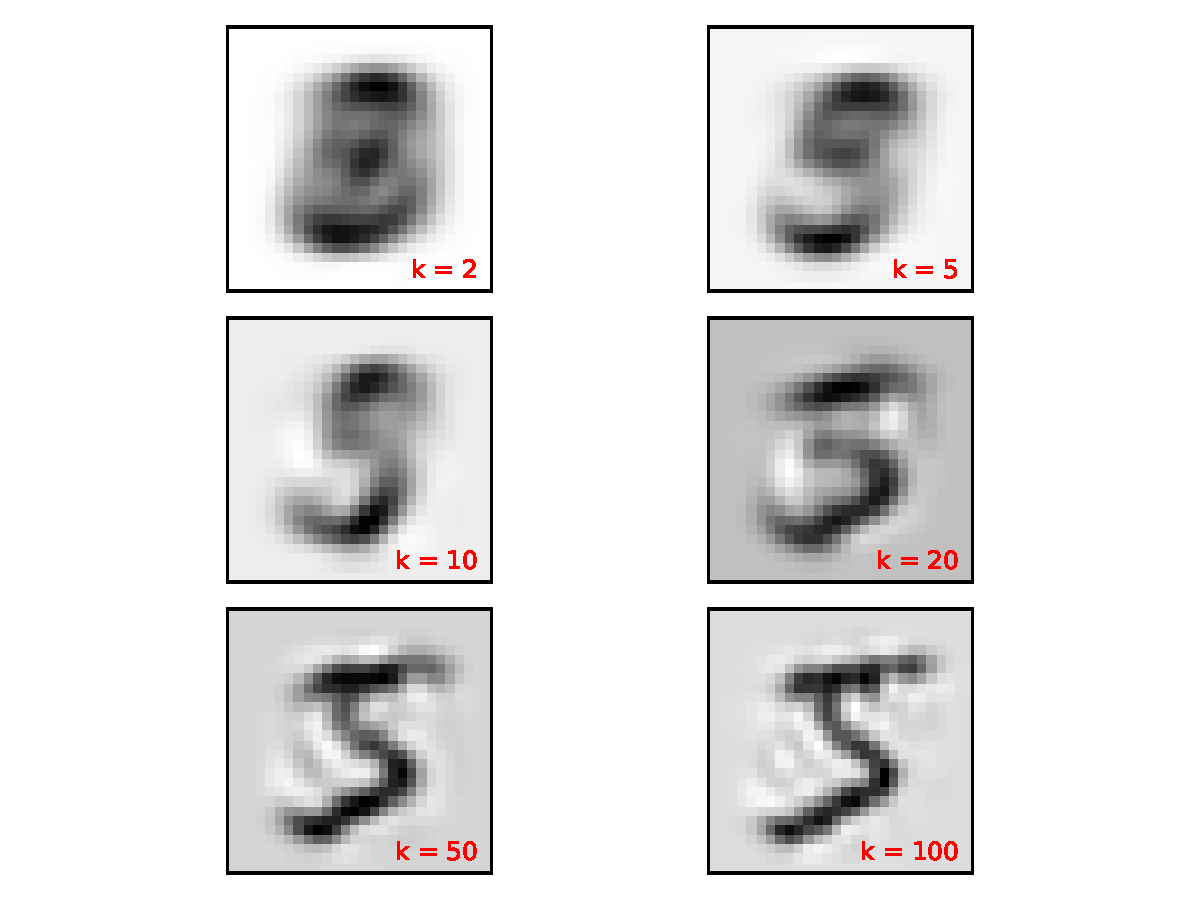
\includegraphics[width=\columnwidth]{5_recon_mnist.pdf}
    \caption{Reconstruction of a number 5 from the MNIST data set (see Fig.~\ref{fig:mnist_digits} using $k \in [2,5,10,20,50,100]$ principal components where the given $k$ is denoted in red in the lower-righthand corner of the respective subplot.}
    \label{fig:recon_5}
\end{figure}

\begin{figure}[H]
	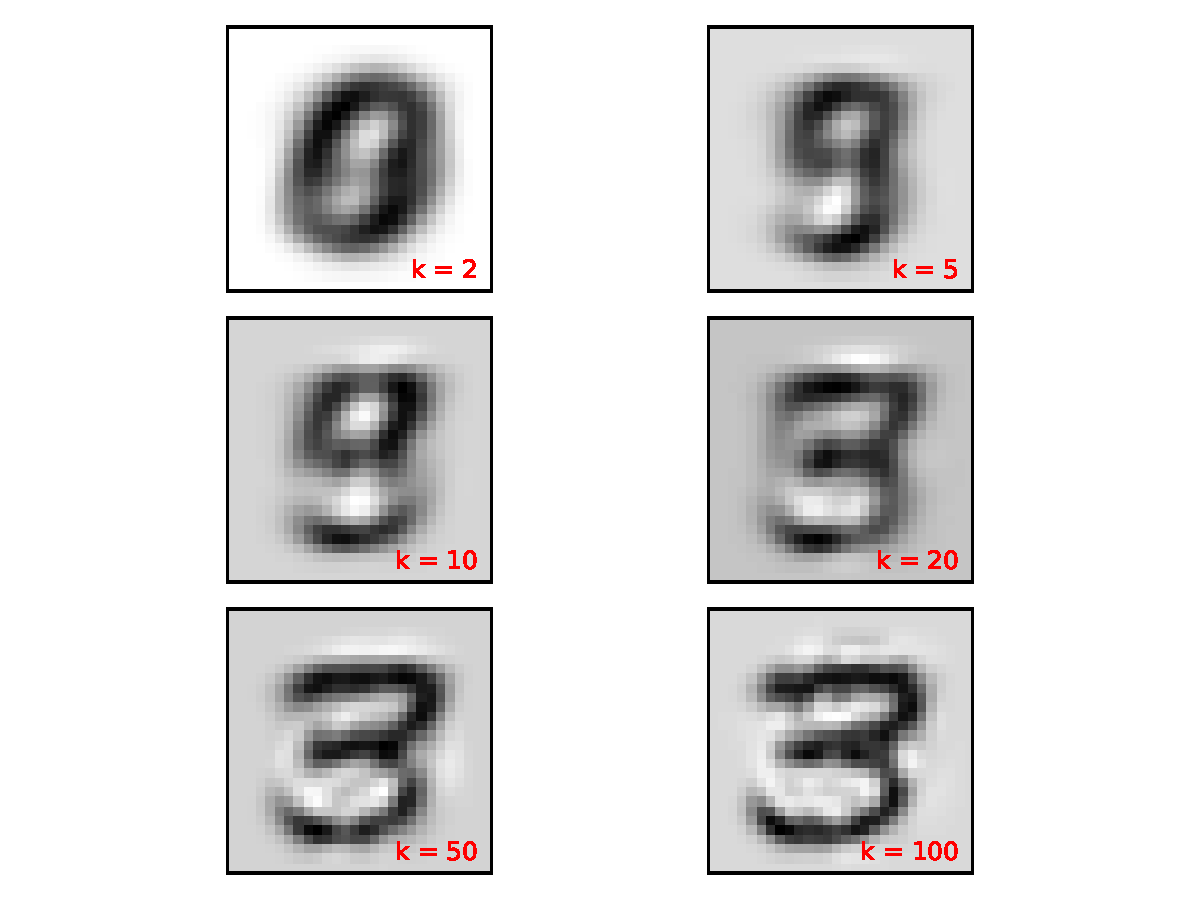
\includegraphics[width=\columnwidth]{3_recon_mnist.pdf}
    \caption{Reconstruction of a number 3 from the MNIST data set (see Fig.~\ref{fig:mnist_digits}) using $k \in [2,5,10,20,50,100]$ principal components where the given $k$ is denoted in red in the lower-righthand corner of the respective subplot.}
    \label{fig:recon_3}
\end{figure}

\begin{figure}[H]
	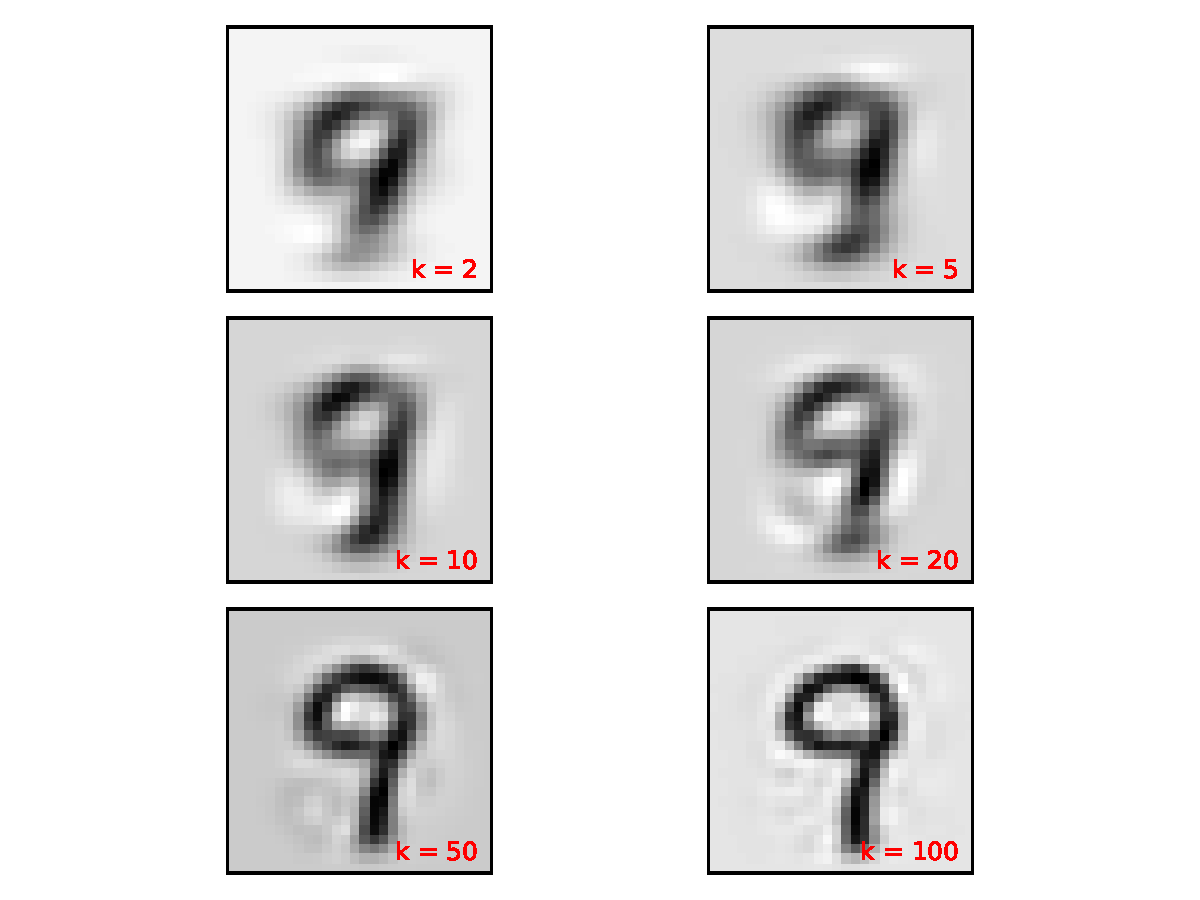
\includegraphics[width=\columnwidth]{9_recon_mnist.pdf}
    \caption{Reconstruction of a number 9 from the MNIST data set (see Fig.~\ref{fig:mnist_digits}) using $k \in [2,5,10,20,50,100]$ principal components where the given $k$ is denoted in red in the lower-righthand corner of the respective subplot.}
    \label{fig:recon_9}
\end{figure}

\begin{figure}[H]
	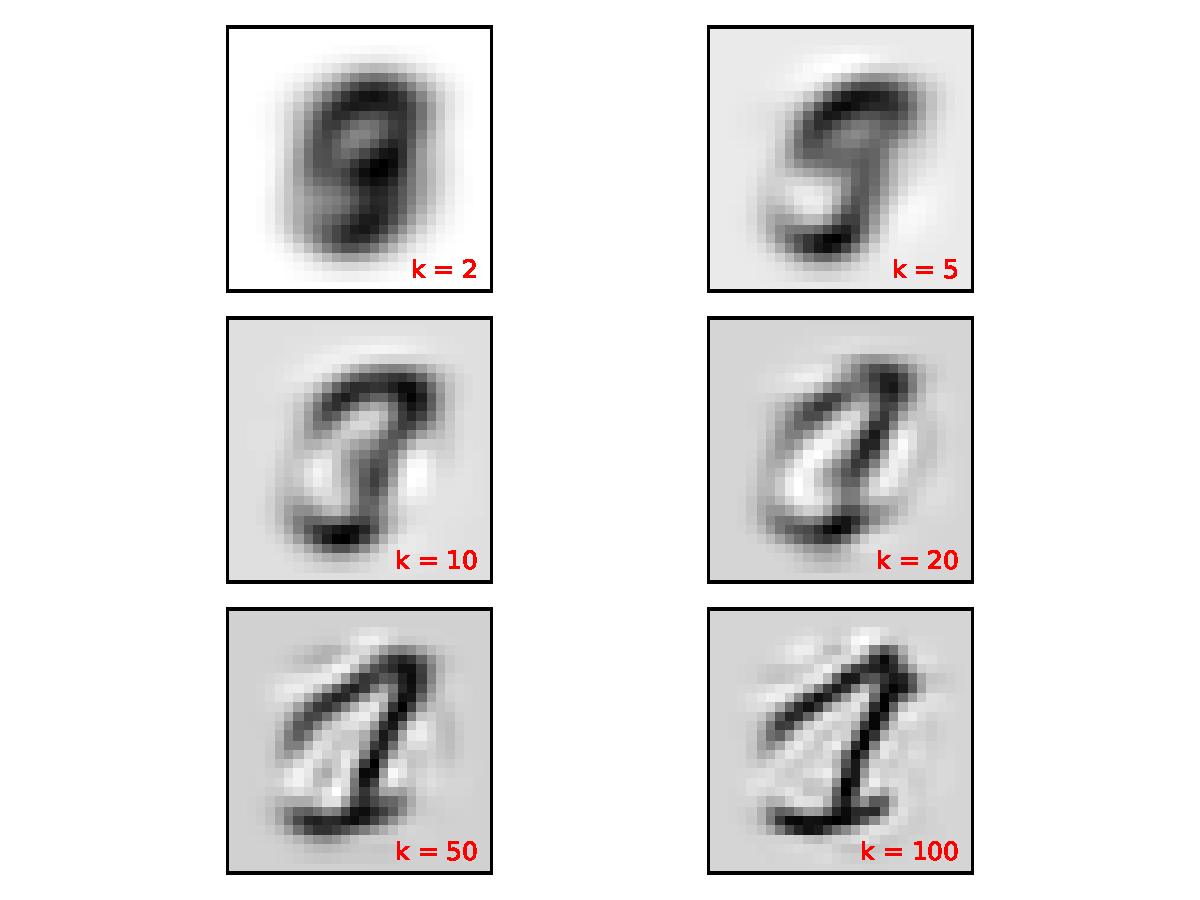
\includegraphics[width=\columnwidth]{1_recon_mnist.pdf}
    \caption{Reconstruction of a number 1 from the MNIST data set (see Fig.~\ref{fig:mnist_digits}) using $k \in [2,5,10,20,50,100]$ principal components where the given $k$ is denoted in red in the lower-righthand corner of the respective subplot.}
    \label{fig:recon_1}
\end{figure}

\begin{figure}[H]
	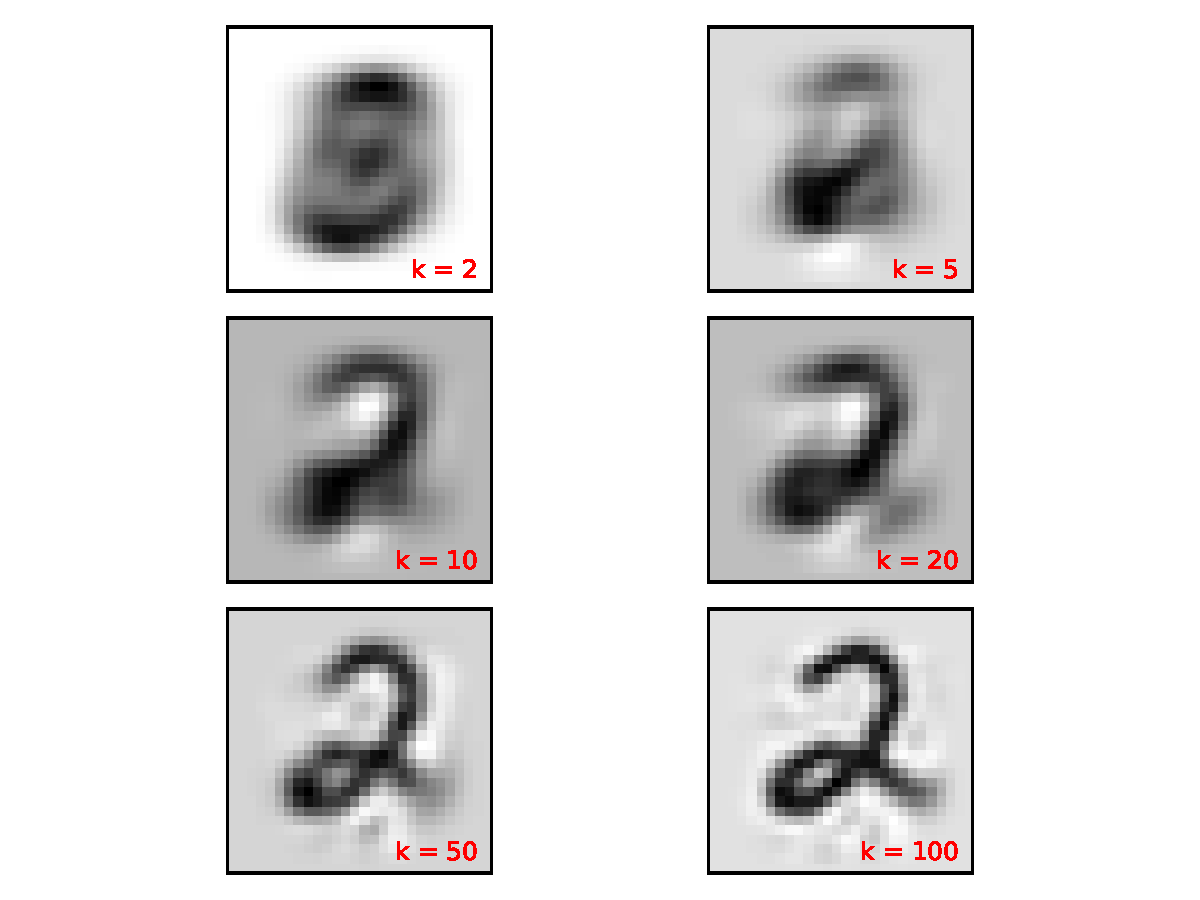
\includegraphics[width=\columnwidth]{2_recon_mnist.pdf}
    \caption{Reconstruction of a number 2 from the MNIST data set (see Fig.~\ref{fig:mnist_digits}) using $k \in [2,5,10,20,50,100]$ principal components where the given $k$ is denoted in red in the lower-righthand corner of the respective subplot.}
    \label{fig:recon_2}
\end{figure}

\begin{figure}[H]
	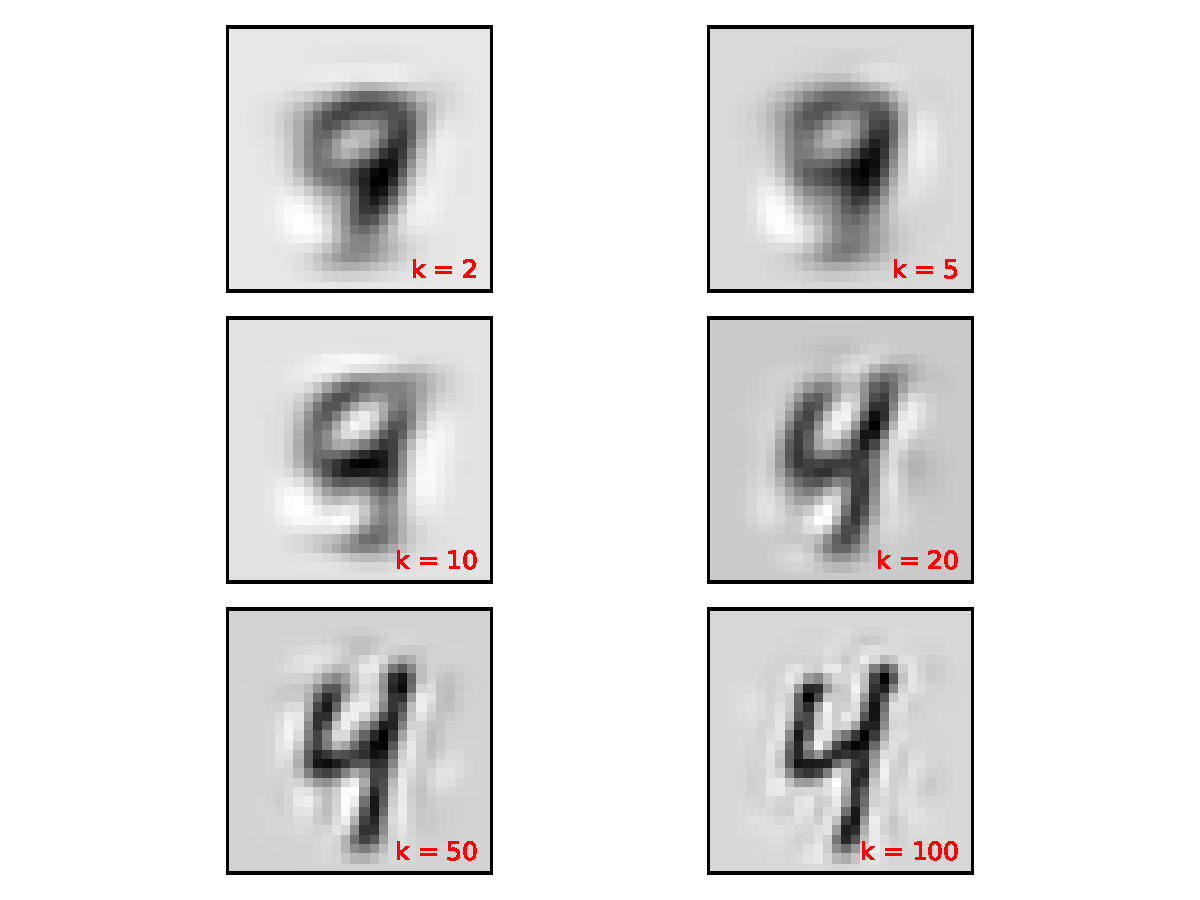
\includegraphics[width=\columnwidth]{4_recon_mnist.pdf}
    \caption{Reconstruction of a number 4 from the MNIST data set (see Fig.~\ref{fig:mnist_digits}) using $k \in [2,5,10,20,50,100]$ principal components where the given $k$ is denoted in red in the lower-righthand corner of the respective subplot.}
    \label{fig:recon_4}
\end{figure}

\subsubsection*{1.4.3}

Broadly, the images reconstructed using at least $k = 20$ principal components appear to be a good, albeit grainy, approximation of the true image.  Some images, in particular the reconstructed 9 and 5, are decently approximated using 10 principal components.  Other digits that have large scatter in how they are drawn, such as 4s, require more principal components to adequately approximate the true image.  All digits reconstructed with at least 50 principal components are good approximations of the original images.  As expected, the more principal components used, the better the approximation becomes since as $k \rightarrow d$, we expect the reconstruction to become equal to the original $X$.



\end{document}